\section{Análisis de diferentes soluciones propuestas}
Vamos a proponer dos escenarios posibles para poder analizar sus soluciones. Estos dos escenarios los vamos a presentar mediante un gráfico cada uno,
donde el tiempo de visualizacion de Scaloni es representado con el color turquesa, y el de los ayudantes es representado con el color azul.
\begin{figure}[H]
    \centering
    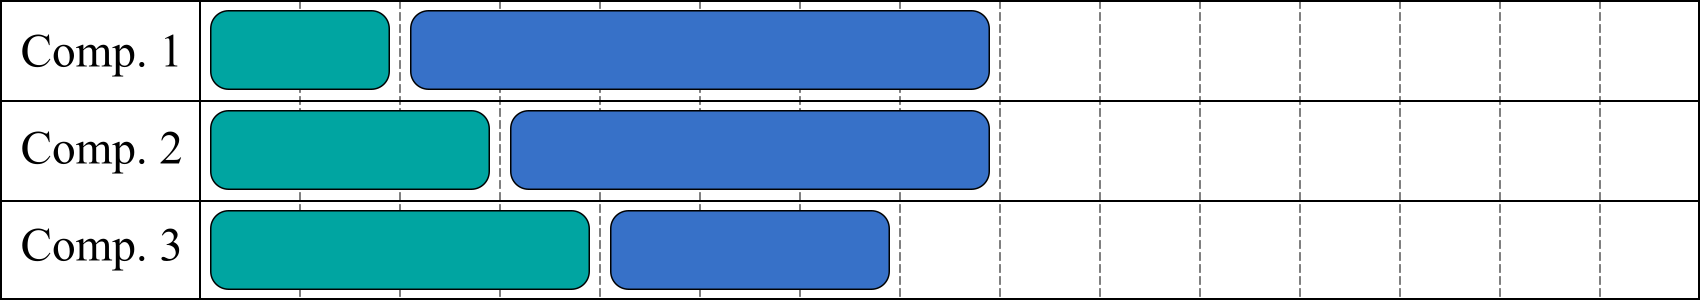
\includegraphics[width=1\textwidth]{img/caso-1.png}
    \caption{El tiempo que le tarda a los ayudantes ver cada compilado es inversamente proporcional a lo que le tarda a Scaloni.}
    \label{fig:Caso 1}
\end{figure}


\begin{figure}[H]
    \centering
    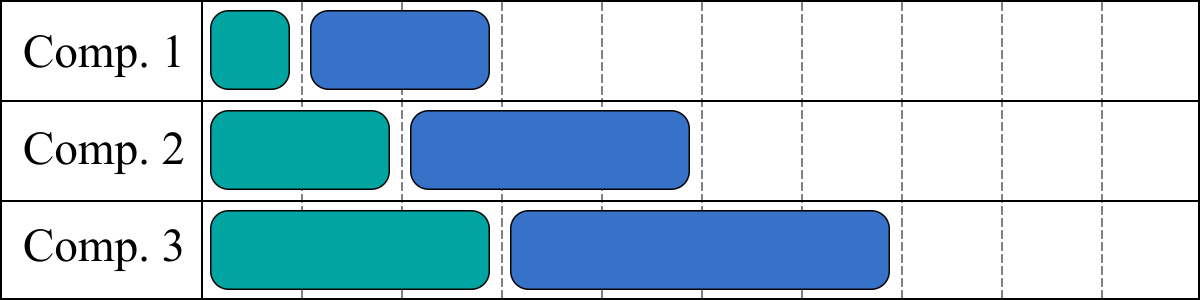
\includegraphics[width=1\textwidth]{img/caso-2.png}
    \caption{El tiempo que le tarda a los ayudantes ver cada compilado es proporcional a lo que le tarda a Scaloni.}
    \label{fig:Caso 2}
\end{figure}

Lo primero que notamos fue que el orden en que Scaloni visualiza los compilados no incide 
en el tiempo que le toma a él en finalizar la revisión de los mismos.

\begin{figure}[H]
    \centering
    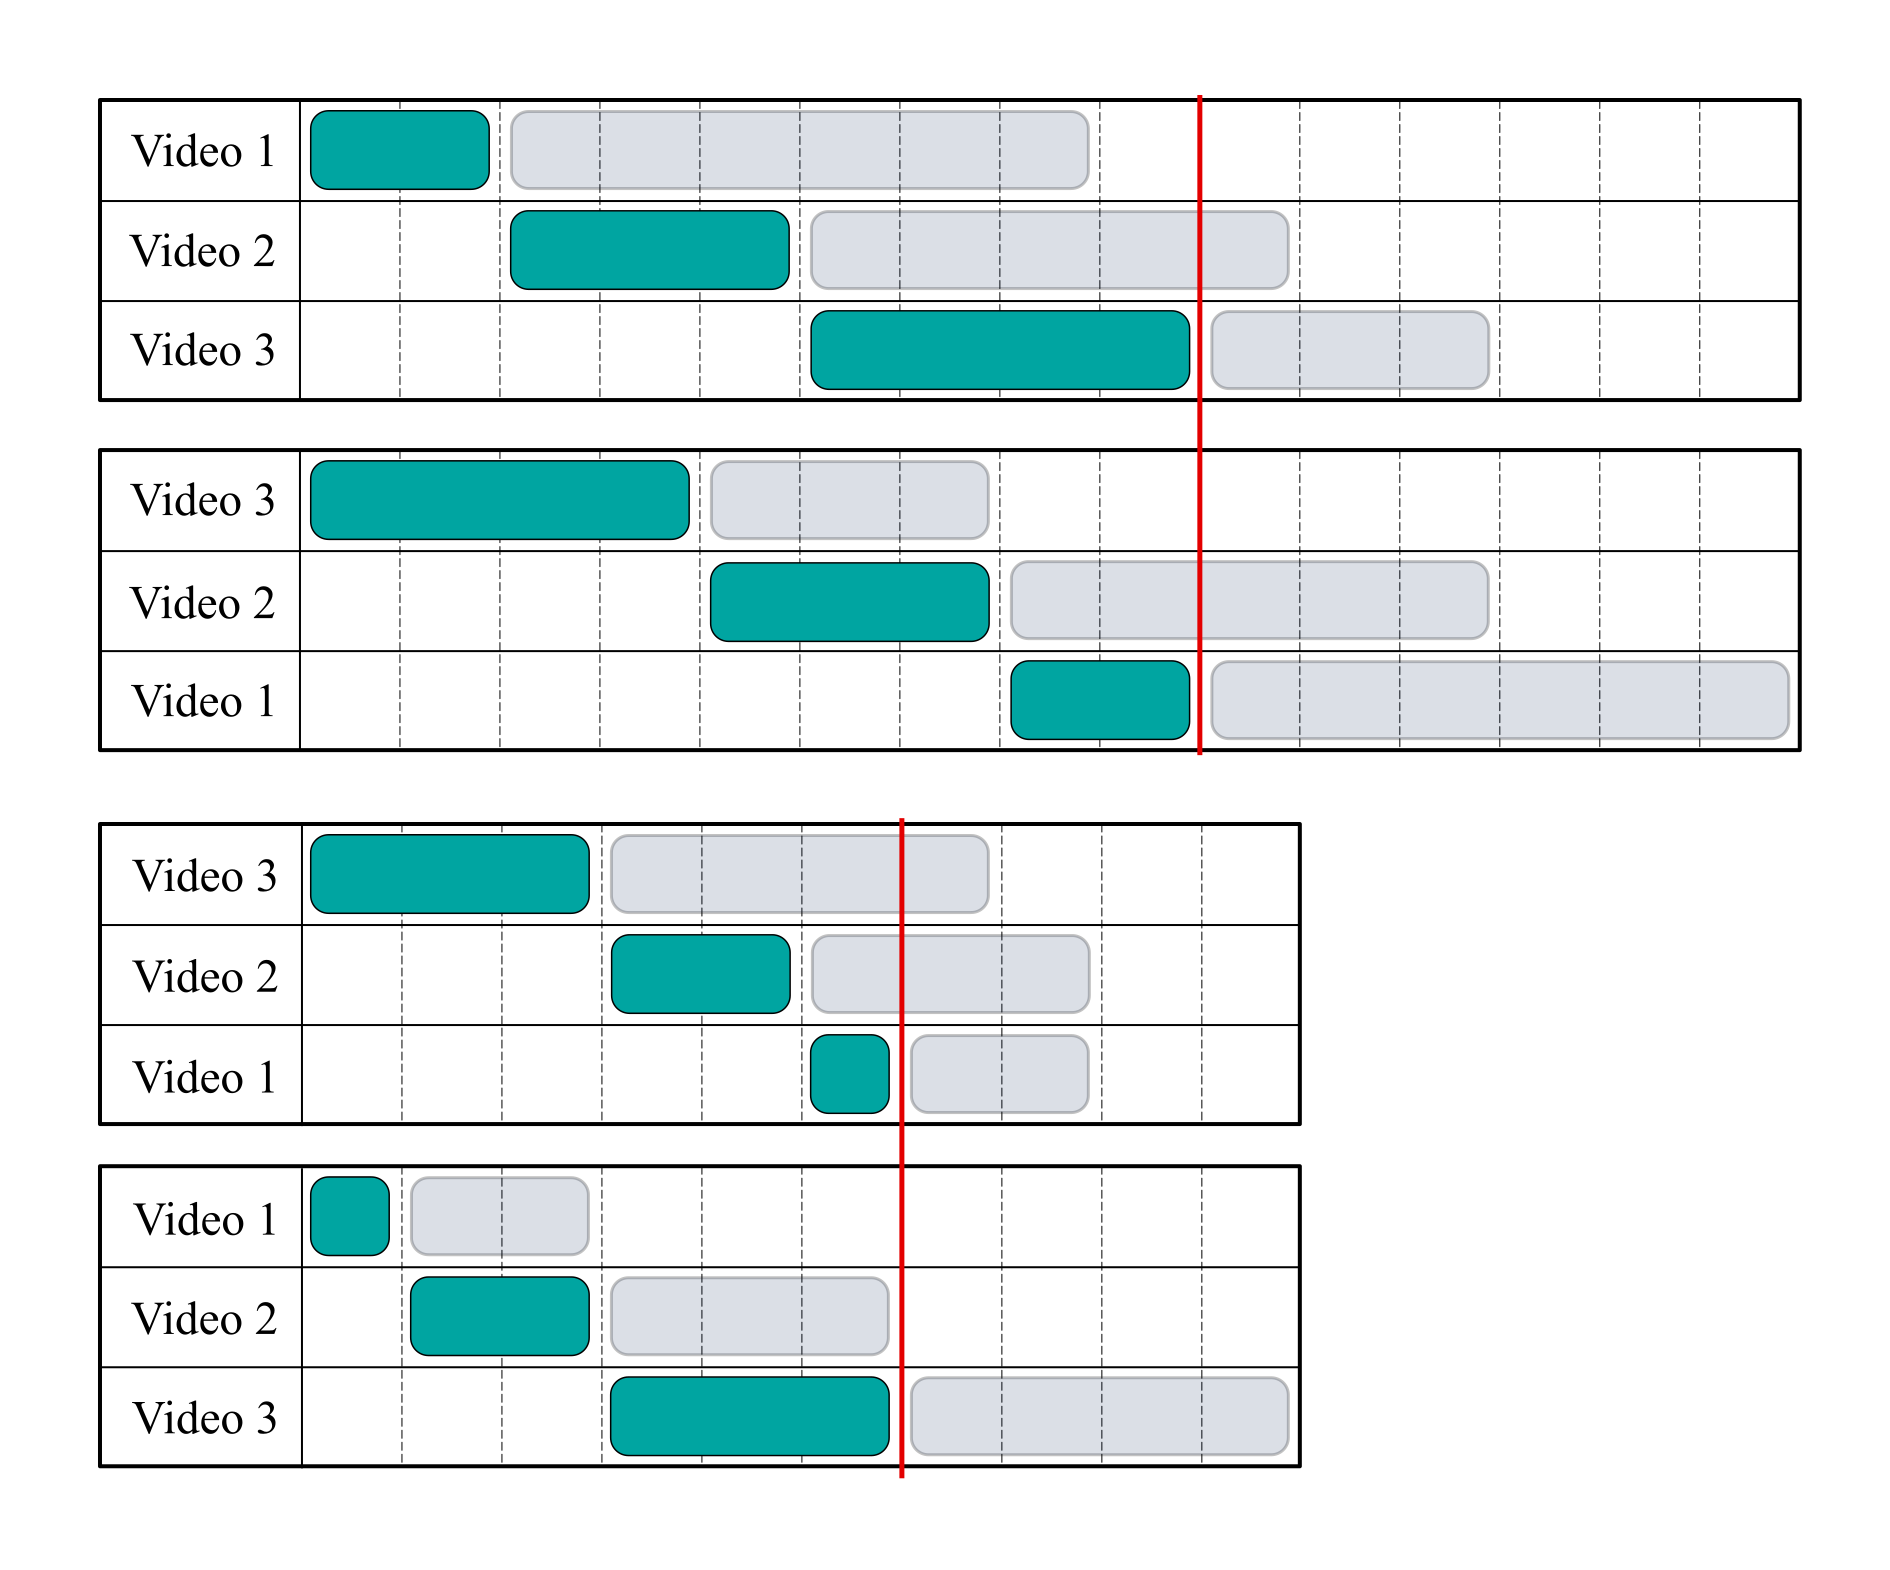
\includegraphics[width=1\textwidth]{img/tiempos-scaloni.png}
    \label{fig:Caso 2}
\end{figure}

Tomando este análisis en consideración, concluimos que el mecanismo de ordenamiento debería únicamente depender
de $a_i$ y no de $s_i$.

\section{Posibles algoritmos}

Posterior a nuestro análisis, propusimos dos algoritmos:

\subsection{Ordenando por $a_i$ de forma creciente}
Este algorítmo sigue las siguientes indicaciones:
\begin{itemize}
    \item Ordenar los compilados de menor a mayor tiempo de análisis por parte de los ayudantes.
    \item Cada vez que termina Scaloni de ver un compilado, inmediatamente un ayudante es asignado a visualizarlo.
\end{itemize}

\subsection{Ordenando por $a_i$ de forma decreciente}
Este algor´ıtmo sigue las siguientes indicaciones:
\begin{itemize}
    \item Ordenar los compilados de mayor a menor tiempo de análisis por parte de los ayudantes.
    \item Cada vez que termina Scaloni de ver un compilado, inmediatamente un ayudante es asignado a visualizarlo.
\end{itemize}

Comparemos cómo se desempeñan nuestros dos algorítmos en cada escenario propuesto:

\subsection{Resultados obtenidos del Caso 1}

\begin{figure}[H]
    \centering
    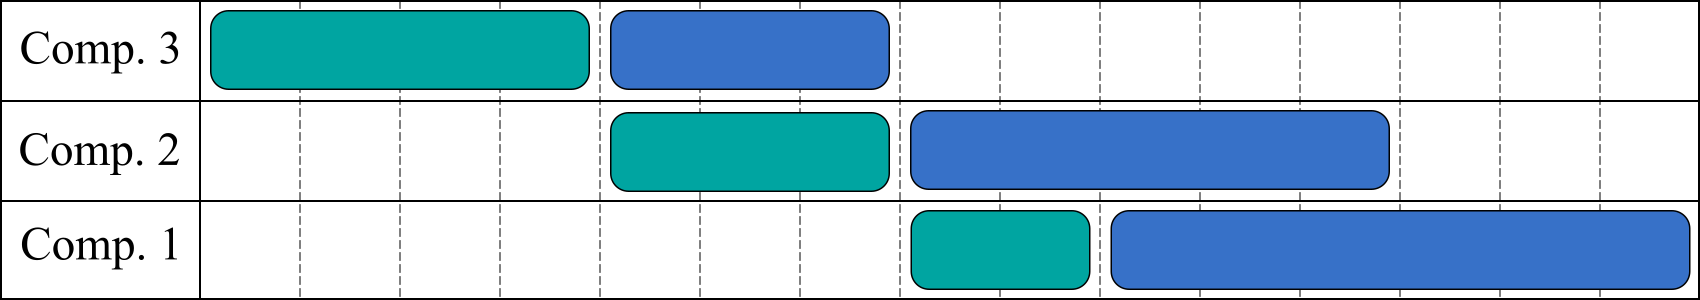
\includegraphics[width=1\textwidth]{img/caso-1-creciente.png}
    \caption{Caso 1 ordenado de forma creciente por $a_i$}
    \label{fig:Caso 1 ordenado de forma creciente por $a_i$}
\end{figure}

\begin{figure}[H]
    \centering
    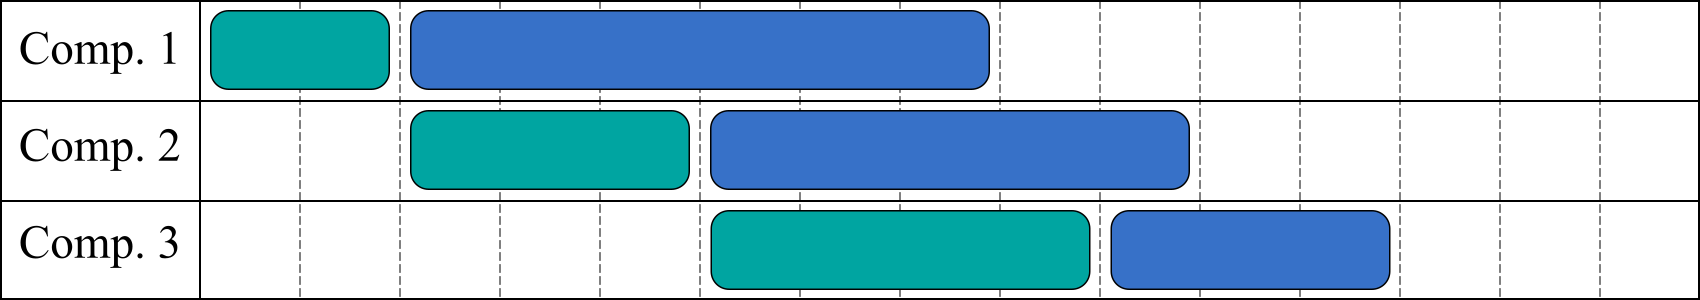
\includegraphics[width=1\textwidth]{img/caso-1-decreciente.png}
    \caption{Caso 1 ordenado de forma decreciente por $a_i$}
    \label{fig:Caso 1 ordenado de forma decreciente por $a_i$}
\end{figure}


\subsection{Resultados obtenidos del Caso 2}

\begin{figure}[H]
    \centering
    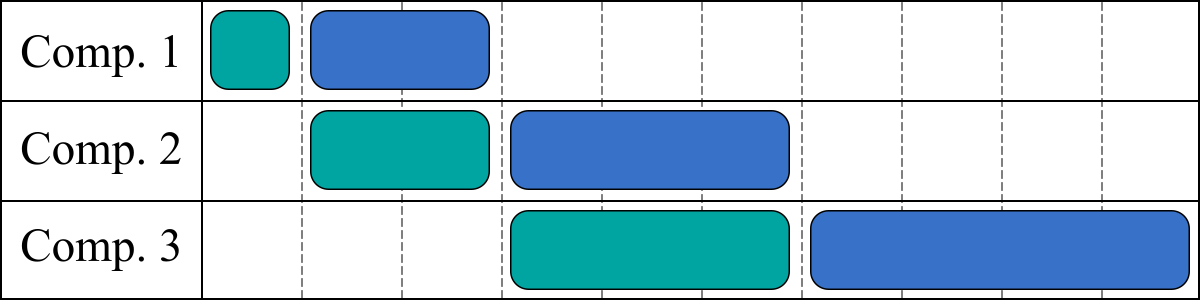
\includegraphics[width=1\textwidth]{img/caso-2-creciente.png}
    \caption{Caso 2 ordenado de forma creciente por $a_i$}
    \label{fig:Caso 2 ordenado de forma creciente por $a_i$}
\end{figure}

\begin{figure}[H]
    \centering
    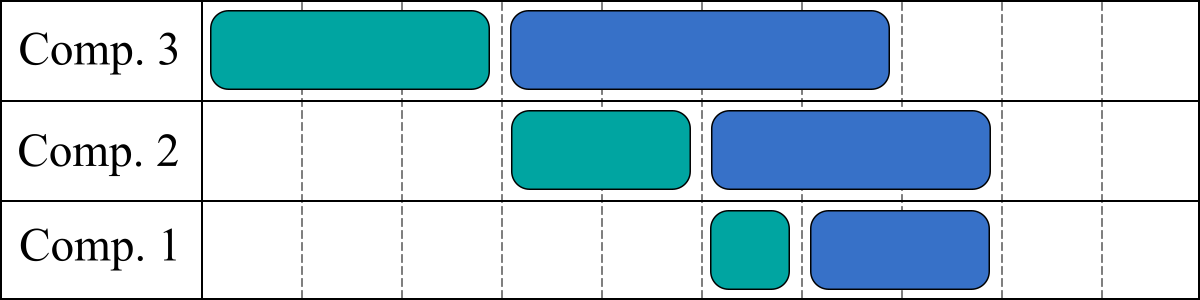
\includegraphics[width=1\textwidth]{img/caso-2-decreciente.png}
    \caption{Caso 2 ordenado de forma decreciente por $a_i$}
    \label{fig:Caso 2 ordenado de forma decreciente por $a_i$}
\end{figure}

Como se puede observar, para ambos casos el ordenamiento decreciente resulta en un tiempo total menor.

\section{Demostración}

Procederemos a demostrar que ordenar los compilados por $a_i$ de forma decreciente minimiza el tiempo total.

Llamamos $C$ al conjunto ordenado de $n$ compilados, $s_i$ el tiempo que le tardar visualizar a Scaloni el $i$-ésimo compilado, y
$a_i$ lo que le tarda a un ayudante. Además, al tiempo que tarda Scaloni analizar los compilados hasta el $k$-ésimo lo representaremos como $S_k$.

$$
S_{k}=\sum_{i=1}^{k}s_{i} 
$$

Luego, el tiempo total que se tarda en analizar los compilados hasta el $k$-ésimo, en el orden
en el que se los presenta, sigue la siguiente formula:


$$
T_{k} = \begin{cases}
s_{1}+a_{1} & k=1 \\
\displaystyle\max{(T_{k-1},S_{k}+a_{k})} & k>1
\end{cases}
$$

Ordenar $C$ para minimizar $T_{n}$ requiere minimizar $\max{(T_{n-1},S_{n}+a_{n})}$. Como $S_{n}$ es independiente del orden de $C$, $S_{n}+a_{n}$ se minimiza colocando último al compilado con el tiempo del ayudante más pequeño. Luego, $T_{n-1}$ se minimiza de la misma manera, resultando en un algoritmo recursivo. Solo nos falta justificar por qué el orden que minimiza $S_{n}+a_{n}$ también minimiza $\max{(T_{n-1},S_{n}+a_{n})}$. Haremos esto partiendo de la asumpción de que se respeta el orden propuesto y de que modificarlo resulta en un $T_n$ más grande.

\begin{itemize}

    \item Si $\max{(T_{n-1},S_{n}+a_{n})} = S_{n}+a_{n}$ ($\implies S_{n}+a_{n} \geq T_{n-1}$)

    Es el caso más trivial, ya que minimizar $S_{n}+a_{n}$ también minimiza $\max{(T_{n-1},S_{n}+a_{n})}$.

    \item Si $\max{(T_{n-1},S_{n}+a_{n})} = T_{n-1}$ ($\implies T_{n-1} \geq S_{n}+a_{n}$)

    Este caso implica que existe un compilado $j$ tal que $a_{j} \geq \sum^{n}_{i=j+1}s_{i}+a_{n} \implies a_{j} > a_{n}$.
    Colocar a este compilado último causaría que $T_{n}'= S_{n}+a_{j}$, y

\end{itemize}

$$
T_{n}' = S_{n}+a_{j}, \ \ \ \  T_{n} = S_{j}+a_{j} 
$$

$$
\begin{aligned}
S_{n} & > S_{j} \\
S_{n} + a_{j}  & > S_{n} + a_{j}  \\
T_{n}' & > T_{n}
\end{aligned}
$$

Esto demuestra que el orden de $C$ que minimiza $T_n$ es con los tiempos $a_i$ decrecientes.


\begin{figure}[H]
    \centering
    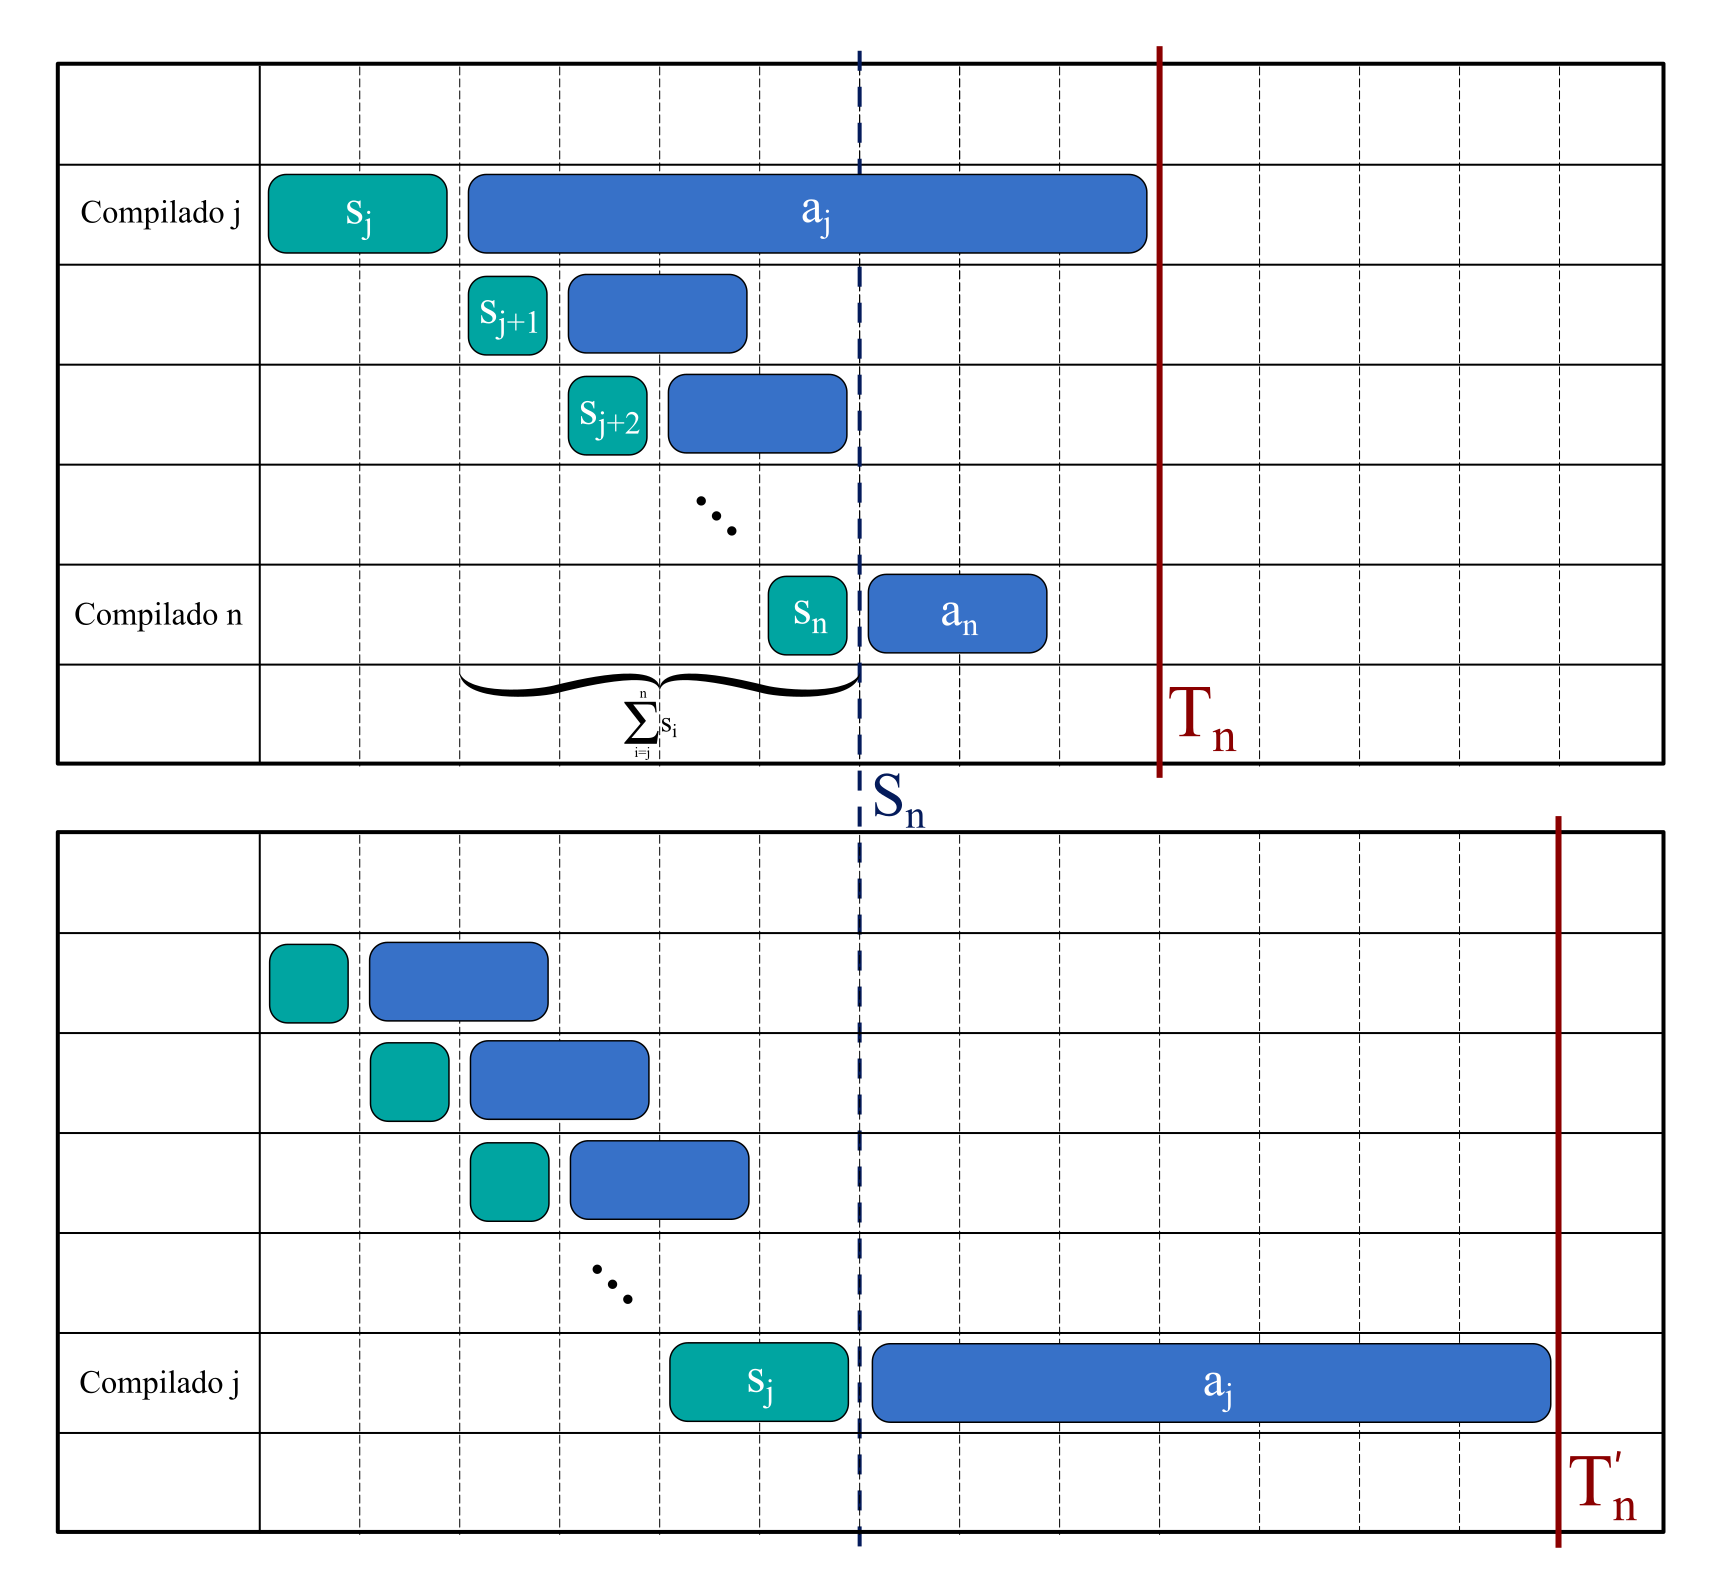
\includegraphics[width=1\textwidth]{img/demostracion.png}
    \caption{Ilustración de la demostración}
    \label{fig:Ilustración de la demostración}
\end{figure}


\textbf{Para ello propusimos el siguiente algoritmo:}

En primer lugar, hemos definido una clase llamada \texttt{Compilado} para modelar el compilado de cada 
oponente, con los atributos \texttt{tiempo\_scaloni} y \texttt{tiempo\_ayudante}, que almacenan 
el tiempo que le lleva analizarlo a Scaloni y a algún ayudante, respectivamente.

\begin{lstlisting}[language=Python]
class Compilado:
    def __init__(self, scaloni, ayudante):
        self.tiempo_scaloni = scaloni
        self.tiempo_ayudante = ayudante
\end{lstlisting}

De esta forma, y teniendo en cuenta los criterios previamente detallados, definimos la función
\texttt{compilados\_ordenados\_de\_forma\_optima} que recibe como parámetro un arreglo con
elementos de la clase \texttt{Compilado}. Esta ordena el arreglo en función del tiempo requerido
por los asistentes para visualizar cada compilado, en orden descendente. 

\begin{lstlisting}[language=Python]
def compilados_ordenados_de_forma_optima(compilados):
    return sorted(compilados, key=lambda compilado: compilado.tiempo_ayudante, reverse=True)
\end{lstlisting}



\begin{itemize}
    \item Los asistentes realizan el análisis de cada uno de los compilados asignados en paralelo. Por lo 
tanto, el tiempo que se invierte en la revisión de un compilado específico de máxima duración, 
puede ser aprovechado de manera tal que este sea visto mientras Scaloni se dedica a la revisión
de otros compilados. De esta forma, nos aseguramos que se minimice el tiempo que suman los ayudantes 
en la resvisión total. 
    \item También en esta solución tiene en consideración el análisis 2 descripto previamente, ya que en el mejor de los casos,
    la $\sum_{k=1}^{n} s_k + a_n$ termina siendo la mínima ya que, por la forma del ordenamiento del algorítmo, $a_n$ es la duración del compilado más corto.

\end{itemize}